\section{Appendix}
\subsection{Example for a Small Delaunay Triangulation}
\label{appendix:DT_def}
    The Delaunay triangulation (DT) is an undirected graph. An edge
    between two nodes \(i\) and \(j\) will be drawn, if there exists
    a circle passing through \(i\) and \(j\), which does not contain
    any other node in its interior.
    \begin{figure}[htbp]
    \centering
        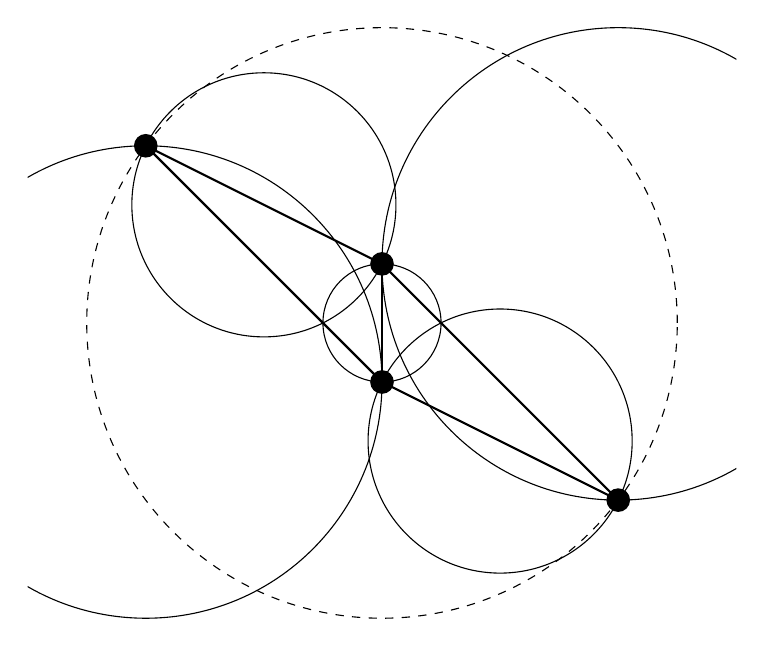
\begin{tikzpicture}[scale=3]
    \clip (-0.5,0) rectangle (2.5,2.5);

    \fill (0, 2  ) circle(0.05);
    \fill (1, 1.5) circle(0.05);
    \fill (1, 1  ) circle(0.05);
    \fill (2, 0.5) circle(0.05);

    \draw[dashed] (1, 1.25)   circle(1.25);
    \draw (2, 1.5)      circle(1);
    \draw (1, 1.25)     circle(0.25);
    \draw (0.5, 1.75)   circle(0.5590);
    \draw (1.5, 0.75)   circle(0.5590);
    \draw (0, 1)        circle(1);

    \draw[thick] (0, 2  ) -- (1, 1.5);
    \draw[thick] (0, 2  ) -- (1, 1  );
    \draw[thick] (1, 1  ) -- (1, 1.5);
    \draw[thick] (1, 1  ) -- (2, 0.5);
    \draw[thick] (1, 1.5) -- (2, 0.5);
\end{tikzpicture}

        \label{sfig:def:DT}
        \caption[Example for a Small Delaunay Triangulation]
        {
            Circles, which contain nodes are dashed.
            Circles, which contain no nodes are not dashed.
            Consequently nodes on the border of not dashed circles are
            connected. Note that the drawn cricles are only examples
            as there there is an infinitive number of alternative not
            dashed circles, which contain no other node.
            Note also that in contrast to the GG the circles do not
            have to be centered on the middle point between the nodes, if
            however, the centered circle does not contain any node, the
            resulting edge will be present in DT and GG. Therefore GG is
            a subgraph of DT.
        }
    \end{figure}

\subsection{Finite Size Effects at the Example of the Specific Heat}
\label{appendix:finiteSizeEffects}
    In Fig.\ \ref{fig:smeared_out_appendix} the specific heat
    \begin{equation}
        c = \frac{N}{T^2}\avg{\avg{E^2} - \avg{E}^2}
    \end{equation}
    is plotted for different system sizes. The finite size effects are obvious.
    The divergence is finite and gets steeper with larger \(L\). Besides
    the maximum moves to the critical temperature with larger \(L\).
    \begin{figure}[htbp]
        \centering
        \includegraphics[width=0.45\textwidth]{plots/Specific_Heat_0}
        \caption[Finite Size Effects by Example of the Specific Heat]
        {
            Effects of different system sizes on the specific heat \(c\)
            at \(\sigma = 0\). Dotted lines are guides to the eye.
        }
        \label{fig:smeared_out_appendix}
    \end{figure}

\subsection{Course of the Critical Temperature $T_c$ with Fixed Coupling Constants $J$}
\label{appendix:fixedCoupling}
    A quick analysis of this model with fixed coupling constants \(J = 1\)
    (i.e.\ \(\alpha=0\)) is performed. The results are displayed in Fig.\ \ref{fig:Tc_deg_A0}.
    The jump from \(\sigma=0\) to \(\sigma>0\) does not disappear as in Fig.\ \ref{fig:Tc_deg}
    for variable \(J\) with \(\alpha=0.5\). This suggests that the
    disappearance of the jump is a random special case for the function
    \(J_{ij}=e^{\alpha(1-d_{ij})}\) at \(\alpha=0.5\).\\
    The simulations were carried out on \(L \in \{16,32,64\}\) lattices
    for a subset of the \(\sigma\) and \(T\) used in the previous simulation.
    Also note that the degree \(K\) is
    the same used in \ref{fig:Tc}\subref{sfig:deg:RNG}\subref{sfig:deg:GG}
    because it is obviously independent of \(J\).
    Further, note that for small values of \(\sigma < 0.3\), \(T_c / K\)
    obtained using the fixed coupling strength \(J=1\) coincides with
    \(T_c / \avg{\sum_{\avg{i,j}}J_{ij}}\) obtained using the distance
    dependent coupling strength, Eq.\ \ref{eq:coupling}.
    This can be expected from the approximate analytic statement presented
    in Sec.\ \ref{sssec:J}.
    \begin{figure}[htbp]
        \centering
        \subfigure[][]
        {
            \label{sfig:Tc:RNG_A0}
            \includegraphics[width=0.45\textwidth]{plots/RNG_Tc_A0}
        }
        \subfigure[][]
        {
            \label{sfig:Tc:GG_A0}
            \includegraphics[width=0.45\textwidth]{plots/GG_Tc_A0}
        }

        \subfigure[][]
        {
            \label{sfig:Tc_norm_deg:RNG_A0}
            \includegraphics[width=0.45\textwidth]{plots/RNG_Tc_norm_deg_A0}
        }
        \subfigure[][]
        {
            \label{sfig:Tc_norm_deg:GG_A0}
            \includegraphics[width=0.45\textwidth]{plots/GG_Tc_norm_deg_A0}
        }

        \caption[Critical Temperature and Critical Temperature Normalized by Degree of the Graph for Fixed Coupling Constants $J=1$]
        {
            Top: Critical Temperature \(T_c\) of the graph over different
            disorder parameters \(\sigma\) with fixed coupling constants \(J=1\) for
            \subref{sfig:deg:RNG} the RNG and
            \subref{sfig:deg:GG} the GG.\\
            Bottom: Critical temperatures normalized by degree \(K\) over
            different disorder parameters \(\sigma\) with fixed coupling constants \(J=1\) for
            \subref{sfig:Tc_norm_deg:RNG} the RNG and
            \subref{sfig:Tc_norm_deg:GG} the GG. The values of \(T_c / K\)
            are compared to those of \(T_c /  \avg{\sum_{\avg{i,j}}J_{ij}}\)
            from Sec.\ \ref{sssec:J}.
        }
        \label{fig:Tc_deg_A0}
    \end{figure}\\
